% VARIABLES
\def\version{1.0.0}

\documentclass[12pt]{article}
\usepackage[inner=2.1cm, bottom=1.5cm, top=1.5cm, outer=2.1cm,
  headheight=24pt, % as per the warning by fancyhdr
  includehead,includefoot,
  heightrounded]{geometry}
% Set the font
\usepackage{helvet}
\renewcommand{\familydefault}{\sfdefault}
% urls
\usepackage[hidelinks]{hyperref}
% disable indent
\usepackage[skip=1em, indent=0pt]{parskip}
% shifted environment
\newenvironment{content}%
  {\list{}{\leftmargin=2cm}\item[]}%
  {\endlist}
% cell color
\usepackage[table, dvipsnames]{xcolor}
% drawings
\usepackage{tikz}
\usepackage{pgfplots}
\pgfplotsset{compat=1.18}
\usetikzlibrary{shapes.geometric,angles,quotes}
\usetikzlibrary{arrows.meta}
\usetikzlibrary{positioning}
\usetikzlibrary{babel}
\usetikzlibrary{fit}
\usetikzlibrary{angles, quotes}
\tikzset{
% Define standard arrow tip
>={Latex[scale=1.25]}
}
\usepackage{tikz-layers}
% floating figures
\usepackage{float}
% do computations
\usepackage{calc}
% advanced tables
\usepackage{makecell}
\usepackage{tabularx}
\usepackage{multirow}
\usepackage{graphicx}
\setlength{\tabcolsep}{10pt}
\renewcommand{\arraystretch}{1.5}
% Functional requirement environment
\newlength{\reqtablelength}
\setlength{\reqtablelength}{0.9\textwidth}
\newcommand{\reqcolor}{Orchid}
\newcommand{\req}[4]{
  \begin{center}
  {
    \vspace{0.5em}
    \small
    \begin{tabularx}{\reqtablelength}{|l|X|}
      \hline
      \cellcolor{\reqcolor!30}\textbf{ID} & #1\\
      \hline
      \hline
      \cellcolor{\reqcolor!15}\textbf{Description} & \cellcolor{\reqcolor!5}\makecell[l]{#2} \\
      \hline
      \cellcolor{\reqcolor!15}\textbf{Rationale} & \cellcolor{\reqcolor!5}\makecell[l]{#3} \\
      \hline
      \cellcolor{\reqcolor!15}\textbf{Refers to} & \cellcolor{\reqcolor!5}\makecell[l]{#4} \\
      \hline
    \end{tabularx}
    \vspace{0.5em}
  }
  \end{center}
}
% User requirement 
\newlength{\ureqtablelength}
\setlength{\ureqtablelength}{0.9\textwidth}
\newcommand{\ureqcolor}{JungleGreen}
\newcommand{\ureq}[2]{
  \begin{center}
  {
    \vspace{0.5em}
    \small
    \begin{tabularx}{\ureqtablelength}{|l|X|}
      \hline
      \cellcolor{\ureqcolor!30}\textbf{ID} & #1\\
      \hline
      \hline
      \cellcolor{\ureqcolor!15}\textbf{Description} & \cellcolor{\ureqcolor!5}#2 \\
      \hline
    \end{tabularx}
  }
  \end{center}
}
% External interface requirement
\newlength{\ireqtablelength}
\setlength{\ireqtablelength}{0.9\textwidth}
\newcommand{\ireqcolor}{orange}
\newcommand{\ireq}[4]{
  \begin{center}
  {
    \vspace{0.5em}
    \small
    \begin{tabularx}{\ireqtablelength}{|l|X|}
      \hline
      \cellcolor{\ireqcolor!30}\textbf{ID} & #1\\
      \hline
      \hline
      \cellcolor{\ireqcolor!15}\textbf{Description} & \cellcolor{\ireqcolor!5}#2 \\
      \hline
      \cellcolor{\ireqcolor!15}\textbf{Rationale} & \cellcolor{\ireqcolor!5}\makecell[l]{#3} \\
      \hline
      \cellcolor{\ireqcolor!15}\textbf{Refers to} & \cellcolor{\ireqcolor!5}\makecell[l]{#4} \\
      \hline
    \end{tabularx}
    \vspace{0.5em}
  }
  \end{center}
}



% Configure headers and footers
\usepackage{fancyhdr}
\renewcommand{\headrulewidth}{1pt}
\renewcommand{\footrulewidth}{1pt}
\renewcommand{\headruleskip}{4pt}
\renewcommand{\footruleskip}{4pt}
\fancyhead{}\fancyfoot{}
\fancyhead[HL]{\scriptsize{\textbf{Educational Computer Architecture Platform 5} \\
ECAP5-DPROC RISC-V processor}}
\fancyhead[HR]{\scriptsize{Page \thepage \\
}}
\fancyfoot[FL]{\scriptsize{Architecture Document}}
\fancyfoot[FR]{\scriptsize{Issue Date: \today}}
\fancyfoot[FC]{\scriptsize{\vspace{1em}\textit{Revision \version}}}


\begin{document}
\begin{titlepage}

\large{\textbf{ECAP5-DPROC}}

\vspace{-0.5em}

\normalsize{RISC-V processor}

\vspace{1.5em}

\Huge{\textbf{Architecture Document}}

\normalsize{\textbf{Revision: \version}}

\normalsize{\textbf{Issue Date: \today}}

\vspace*{\fill}

{\scriptsize \parindent0pt \itshape
Copyright (C) Clément Chaine

ECAP5-DPROC is free software: you can redistribute it and/or modify it under the terms of the GNU General Public License as published by the Free Software Foundation, either version 3 of the License, or (at your option) any later version.

ECAP5-DPROC is distributed in the hope that it will be useful, but WITHOUT ANY WARRANTY; without even the implied warranty of MERCHANTABILITY or FITNESS FOR A PARTICULAR PURPOSE. See the GNU General Public License for more details.

\vspace{-0.5em}

You should have received a copy of the GNU General Public License along with ECAP5-DPROC. If not, see \textnormal{\url{http://www.gnu.org/licenses/}}}

\vspace{1em}

\par\noindent\rule{\textwidth}{1pt}

\end{titlepage}

\newpage

\pagestyle{fancy}
\normalsize
\tableofcontents
\newpage
\section{Introduction}
\subsection{Scope}
\begin{content}
This is the Architecture Document for the ECAP5-DPROC, a RISC-V implementation targeting ECAP5 (\textit{Educational Computer Architecture Platform 5}). Included in this documents are a description of the features, functional partitionning as well as descriptions of the functional blocks of the system.

This document is updated as appropriate. Please check \url{https://github.com/cchaine/ECAP5-DPROC} for the latest revision of this document.
\end{content}

\subsection{Overview Description}
\begin{content}
ECAP5-DPROC implements the RV32I instruction set described in the \textit{The RISC-V Instruction Set Manual} through a 5 stage pipeline.

\textit{\textbf{To Be Completed}}
\end{content}

\newpage

\section{Overall Description}

\subsection{User needs}

\begin{content}
ECAP5 is the primary user for ECAP5-DPROC. ECAP5-DPROC could however be used as a standalone RISC-V processor. The following requirements define the user needs. 
\end{content}

\ureq{U\_INSTRUCTION\_SET\_01}{
  ECAP5-DPROC shall implement the RV32I instruction set.
}

\begin{content}
  In order to improve the usability of ECAP5-DPROC, it shall have a \textit{von Neumann} architecture as it only requires one memory interface.
\end{content}

\ureq{U\_MEMORY\_INTERFACE\_01}{
  ECAP5-DPROC shall access both instructions and data through a unique memory interface.
}

\ureq{U\_MEMORY\_INTERFACE\_02}{
  ECAP5-DPROC's unique memory interface shall be compliant with the AXI-Lite specification.
}

\ureq{U\_RESET\_01}{
  ECAP5-DPROC shall provide a signal which shall hold ECAP5-DPROC in a reset state while asserted.
}

\begin{content}
The polarity of the reset signal mentionned in \texttt{U\_RESET\_01} is not specified by the user.
\end{content}

\ureq{U\_BOOT\_ADDRESS\_01}{
  The address at which ECAP5-DPROC jumps after the reset signal is deasserted shall be hardware-configurable.
}

\begin{content}
The address mentionned in \texttt{U\_BOOT\_ADDRESS\_01} can be either configured through hardware signals or can be selected at compile-time.
\end{content}

\ureq{U\_HARDWARE\_INTERRUPT\_01}{
  ECAP5-DPROC shall provide an signal which shall interrupt ECAP5-DPROC's execution flow while asserted.
}

\ureq{U\_HARDWARE\_INTERRUPT\_02}{
  ECAP5-DPROC shall jump to a software-configurable address when it is interrupted.
}

\begin{content}
The memory address at which ECAP5-DPROC shall jump to when interrupted is not specified by the user.
\end{content}

\ureq{U\_DEBUG\_01}{
  ECAP5-DPROC shall be compliant with the RISC-V External Debug Support specification.
}

\begin{content}
There is no performance goal required by ECAP5 for ECAP5-DPROC as ECAP5 is an educational platform.
\end{content}

\subsection{Assumptions and Dependencies}

\begin{content}
Describe what the assumptions for the product are : Targeting the ecp5 family, based around opensource toolchains.
\end{content}

\section{Requirements}

\subsection{External Interface Requirements}

\begin{figure}[h!]
    \centering
    \scalebox{0.85}{
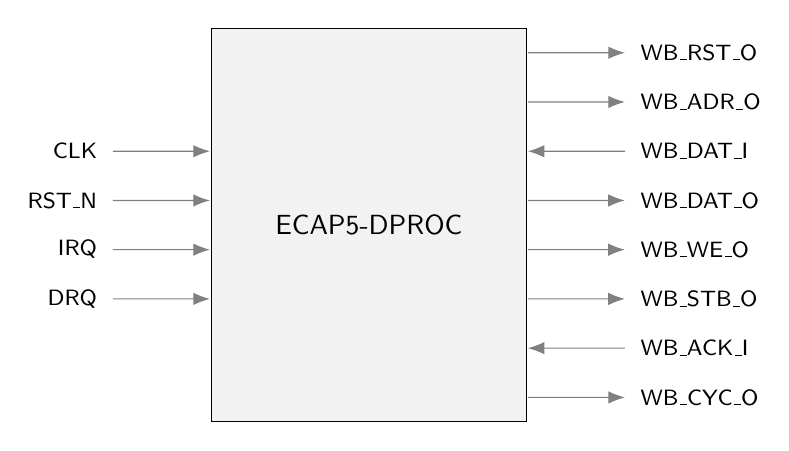
\begin{tikzpicture}[scale=1.25, draw=gray, inner sep=0, outer sep=0]
  \node[rectangle, draw=black,
    minimum height = 5cm,
    minimum width = 4cm,
    fill = gray!10] (box) at (0, 0) {ECAP5-DPROC};

  % left
  \node (lport1) at ([yshift=0.75cm]box.west) {};
  \node (lport2) at ([yshift=0.25cm]box.west) {};
  \node (lport3) at ([yshift=-0.25cm]box.west) {};
  \node (lport4) at ([yshift=-0.75cm]box.west) {};

  \draw[->] ([xshift=-1cm]lport1.center) node[left=0.2cm, anchor=east]{\footnotesize CLK} -- (lport1);
  \draw[->] ([xshift=-1cm]lport2.center) node[left=0.2cm, anchor=east]{\footnotesize RST\_N} -- (lport2);
  \draw[->] ([xshift=-1cm]lport3.center) node[left=0.2cm, anchor=east]{\footnotesize IRQ} -- (lport3);
  \draw[->] ([xshift=-1cm]lport4.center) node[left=0.2cm, anchor=east]{\footnotesize DRQ} -- (lport4);

  % right
  \node (rport4) at ([yshift=0.25cm]box.east) {};
  \node (rport3) at ([yshift=0.5cm]rport4.center) {};
  \node (rport2) at ([yshift=0.5cm]rport3.center) {};
  \node (rport1) at ([yshift=0.5cm]rport2.center) {};

  \node (rport5) at ([yshift=-0.25cm]box.east) {};
  \node (rport6) at ([yshift=-0.5cm]rport5.center) {};
  \node (rport7) at ([yshift=-0.5cm]rport6.center) {};
  \node (rport8) at ([yshift=-0.5cm]rport7.center) {};

  \draw[<-] ([xshift=1cm]rport1.center) node[right=0.2cm, anchor=west]{\footnotesize WB\_RST\_O} -- (rport1);
  \draw[<-] ([xshift=1cm]rport2.center) node[right=0.2cm, anchor=west]{\footnotesize WB\_ADR\_O} -- (rport2);
  \draw[->] ([xshift=1cm]rport3.center) node[right=0.2cm, anchor=west]{\footnotesize WB\_DAT\_I} -- (rport3);
  \draw[<-] ([xshift=1cm]rport4.center) node[right=0.2cm, anchor=west]{\footnotesize WB\_DAT\_O} -- (rport4);
  \draw[<-] ([xshift=1cm]rport5.center) node[right=0.2cm, anchor=west]{\footnotesize WB\_WE\_O} -- (rport5);
  \draw[<-] ([xshift=1cm]rport6.center) node[right=0.2cm, anchor=west]{\footnotesize WB\_STB\_O} -- (rport6);
  \draw[->] ([xshift=1cm]rport7.center) node[right=0.2cm, anchor=west]{\footnotesize WB\_ACK\_I} -- (rport7);
  \draw[<-] ([xshift=1cm]rport8.center) node[right=0.2cm, anchor=west]{\footnotesize WB\_CYC\_O} -- (rport8);
\end{tikzpicture}
}

    \caption{Schematic view of the external interface of ECAP5-DPROC}
    \label{fig:externalinterface}
\end{figure}

\begin{table}[H]
  \centering
  {
\footnotesize
\begin{tabularx}{0.9\textwidth}{|l|c|c|X|}
  \hline
  \cellcolor{gray!20}\textbf{NAME} & \cellcolor{gray!20}\textbf{TYPE} & \cellcolor{gray!20}\textbf{WIDTH} & \cellcolor{gray!20}\textbf{DESCRIPTION} \\
  \hline
  CLK & I & 1 & Clock input. \\
  \hline
  RST\_N & I & 1 & Hardware reset. Active low. \\
  \hline
  IRQ & I & 1 & External interrupt request. \\
  \hline
  DRQ & I & 1 & Debug request. \\
  \hline
\end{tabularx}
}

  \caption{ECAP5-DPROC control signals}
  \label{tab:control-interface}
\end{table}

\begin{table}[H]
  \centering
  {
\footnotesize
\begin{tabularx}{0.9\textwidth}{|l|c|c|X|}
  \hline
  \cellcolor{gray!20}\textbf{NAME} & \cellcolor{gray!20}\textbf{TYPE} & \cellcolor{gray!20}\textbf{WIDTH} & \cellcolor{gray!20}\textbf{DESCRIPTION} \\
  \hline
  \multicolumn{4}{|l|}{\textbf{READ ADDRESS BUS}} \\
  \hline
  ARADDR & O & 32 & Read address. \\
  \hline
  ARVALID & O & 1 & Read address valid. \\
  \hline
  ARREADY & I & 1 & Read address ready. \\ 
  \hline
  \multicolumn{4}{|l|}{\textbf{READ DATA BUS}} \\
  \hline
  RDATA & I & 32 & Read data. \\
  \hline
  RRESP & I & 2 & Read response. \\
  \hline
  RVALID & I & 1 & Read valid. \\
  \hline
  RREADY & O & 1 & Read ready. \\ 
  \hline
  \multicolumn{4}{|l|}{\textbf{WRITE ADDRESS BUS}} \\
  \hline
  AWADDR & O & 32 & Write address. \\
  \hline
  AWVALID & O & 1 & Write address valid. \\
  \hline
  AWREADY & I & 1 & Write address ready \\
  \hline
  \multicolumn{4}{|l|}{\textbf{WRITE DATA BUS}} \\
  \hline
  WDATA & O & 32 & Write data. \\
  \hline
  WSTRB & O & 4 & Write strobes. \\
  \hline
  \multicolumn{4}{|l|}{\textbf{WRITE RESPONSE BUS}} \\
  \hline
  BRESP & I & 2 & Write response. \\
  \hline
  BVALID & I & 1 & Write response valid. \\
  \hline
  BREADY & O & 1 & Response ready. \\
  \hline
\end{tabularx}
}

  \caption{ECAP5-DPROC memory interface signals}
  \label{tab:memory-interface}
\end{table}

\ireq{I\_CLK\_01}{
  All inputs and outputs of ECAP5-DPROC shall belong to CLK's clock domain.
}{}

\ireq{I\_RESET\_01}{
  The RST\_N signal shall hold ECAP5-DPROC in a reset state while asserted.
}{
  U\_RESET\_01
}

\ireq{I\_RESET\_02}{
  RST\_N polarity shall be active low.
}{}

\ireq{I\_IRQ\_01}{
  ECAP5-DPROC shall jump to a software-configurable address when input IRQ is asserted.
}{
  U\_HARDWARE\_INTERRUPT\_01, U\_HARDWARE\_INTERRUPT\_02
}

\ireq{I\_DIRQ\_01}{
  TBD
}{}

\ireq{I\_MEMORY\_INTERFACE\_01}{
  Signals from table \ref{tab:memory-interface} shall be compliant with the AXI-Lite specification.
}{
  U\_MEMORY\_INTERFACE\_02
}

\begin{content}
  Behavioral specification for symbols in table \ref{tab:memory-interface} is outlined in the functional requirements section, subsection \ref{spec-memory-interface}.
\end{content}

\subsection{Functional Requirements}

\subsubsection{Instruction decoding}

\req{REQ\_Test\_01}{
  Requirement title
}{
  This is the rationale of the requirement
}{
  This is the refers to of the requirement
}

\subsubsection{Memory interface}
\label{spec-memory-interface}

\begin{content}
  Outline requirements to be compliant with the AXI-Lite specification.
\end{content}

\subsection{Nonfunctional Requirements}

\begin{content}
These can be : performance, safety, security, usability, scalability.
\end{content}

\newpage

\section{Functional Partitioning}

\newpage

\end{document}
